\documentclass[12pt,hyperref=true,mathserif]{beamer}
\usepackage{amsmath}
\usetheme{AnnArbor}
\graphicspath{{Figure/}{figures/}{figure/}{pictures/}{picture/}{pic/}{pics/}}
\begin{document}
\title[CE APA Analysis]{An Analysis of Channel Estimation and Equalization Techniques
Based on Affine Projection Algorithm}
\author{Yanan Xiao}
\institute[NPU]{Northwestern Polytechnic University}
\date[Defense \& Presentation]{Graduation Design Thesis Presentation}

\begin{frame}
\titlepage
\end{frame}
% \begin{frame}
% \frametitle{Glossary}
% \begin{itemize}
%  \item HeHe
%  \item HeiHei
%  \item XiXi
%\end{itemize}
% \end{frame}
\section{Introduction}
\subsection{Outline}
\begin{frame}[shrink]
\frametitle{Outline}
\tableofcontents
\end{frame}

\subsection{Applications}
\begin{frame}
\frametitle{Study in Noisy Environment}
\begin{columns}
\begin{column}{0.5\textwidth}
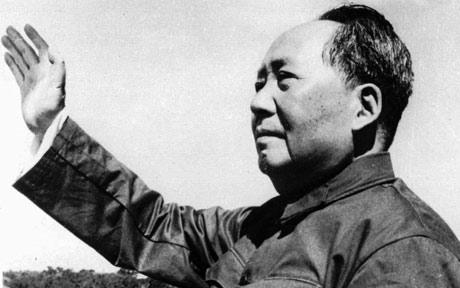
\includegraphics[scale=0.35]{ChairmanMao.jpg}
\end{column}
\begin{column}{0.5\textwidth}
Judge how noisy the channel is---suitable for you to learn, or too noisy.
\end{column}
\end{columns}
\end{frame}

\begin{frame}
\frametitle{Tweet under Supervision}
\begin{columns}
\begin{column}{0.5\textwidth}

\includegraphics[scale=0.45]{HeRundong.jpg}
\end{column}
\begin{column}{0.5\textwidth}
Judge whether it is safe to post something on Weibo.com.
\end{column}
\end{columns}
\end{frame}

\section{Development}
\subsection{Performance Functions}
\begin{frame}
\frametitle{Performance (Cost) Functions}
\begin{itemize}
  \item \textcolor{red}{Mean Square Error}~~$E[e^{2}(n)]$ (Most popular)\\
  \textcolor{blue}{Adaptive algorithms:} Least Mean Square (LMS), Normalized LMS (NLMS),
  Affine Projection (AP), Recursive Least Squares (RLS), etc.

  \item \textcolor{red}{Regularized MSE}
  \begin{equation}\label{equ:RegMSE}
    J_{rms}~=~E[e^{2}(n)]+\alpha \|\mathbf{w}(n)\|^{2}
  \end{equation}
  \textcolor{blue}{Adaptive algorithm:} Leaky Least Mean Square (leaky LMS)
  \item \textcolor{red}{$l_{1}$ norm} criterion
    \begin{equation}\label{equ:Lnorm}
    J_{l_{1}}~=~E[|e(n)|]
  \end{equation}
  \textcolor{blue}{Adaptive algorithm:} Sign-Error
\end{itemize}
\end{frame}

\subsection{Performance (Cost) Functions - continued}
\begin{frame}
\begin{itemize}
  \item \textcolor{red}{Least Mean Fourth (LMF)} criterion
  \begin{equation}\label{equ:LeastMF}
    J_{LMF}~=~E[e^{4}(n)]
  \end{equation}
  \textcolor{blue}{Adaptive algorithm:} Least Mean Fourth (LMF)
  \item \textcolor{red}{Least Mean Mixed Norm (LMMN)} criterion
  \begin{equation}\label{equ:LeastMMN}
    J_{LMMN}~=~E[\alpha e^{2}(n)+\frac{1}{2}(1-\alpha)e^{4}(n)]
  \end{equation}
  \textcolor{blue}{Adaptive algorithm:} Least Mean Mixed Norm (LMMN)
  \item \textcolor{red}{Constant Modulus} criterion
  \begin{equation}\label{equ:ConstantM}
    J_{CM}~=~E[(\gamma-|\mathbf{x}^{T}(n)\mathbf{w}(n)|^{2})^{2}]
  \end{equation}
  \textcolor{blue}{Adaptive algorithm:} Constant Modulus (CM)
\end{itemize}
\end{frame}

\subsection{Affine Projection Algorithm}
\begin{frame}
\frametitle{Affine Projection Algorithm as a Projection onto an Affine Subspace}
\begin{itemize}
  \item[$\bigstar$] Conditions for the analysis
  \item \quad$\mathbf{e}(n)~=~\mathbf{d}(n)-\mathbf{X}^{T}(n)\mathbf{w}(n)$
  \item \quad$\mathbf{d}(n)~=~\mathbf{X}^{T}(n)\mathbf{w}^{0}$ defines the optimal solution in the least squares sense
  \item \quad$\mathbf{v}(n)~=~\mathbf{w}(n)-\mathbf{w}^{0}$ (weight error vector)
  \item[$\bigstar$] Error vector
  \item \quad$\mathbf{e}(n) ~=~ \mathbf{d}(n)~=~\mathbf{X}^{T}(n)[\mathbf{v}(n)+\mathbf{w}(n+1)]$
  \item \qquad\quad$~=~\mathbf{X}^{T}(n)\mathbf{w}(n+1) - \mathbf{X}^{T}(n)[\mathbf{v}(n)+\mathbf{w}(n+1)]$
  \item \qquad\quad$~=~-\mathbf{X}^{T}(n)\mathbf{v}(n)$
\end{itemize}
\end{frame}

\begin{frame}[allowframebreaks,shrink]
\begin{equation}\label{equ:ErrorV}
  \mathbf{e}(n)~=~-\mathbf{X}^{T}\mathbf{v}(n)
\end{equation}
\begin{itemize}
  \item \emph{Interpretation:} To minimize the error $\mathbf{v}(n)$ should be orthogonal to all input vectors\\
  \emph{Restriction:} We are going to use only \{$\mathbf{x}(n)$,$\mathbf{x}(n-1)$,$\ldots$,$\mathbf{x}(n-P)$\}
\end{itemize}
\begin{itemize}
  \item \emph{Iterative solution:} We can subtract from $\mathbf{v}(n)$ onto the range of $\mathbf{X}{n}$ at
  each iteration\\
  \textcolor{blue}{Projection onto an affine subspace}
  \begin{equation}\label{equ:ProjectionOntoSubspace}
  \mathbf{v}(n+1)~=~\mathbf{v}(n)-\mathbf{P}_{\mathbf{X}(n)}\mathbf{v}(n)
  \end{equation}
\end{itemize}
\begin{itemize}
  \item Using $\mathbf{X}^{T}(n)\mathbf{v}(n)~=~-\mathbf{e}(n)$\\
  \textcolor{blue}{AP algorithm}
  \begin{equation}\label{equ:AffineProjectionAlgo}
    \mathbf{v}(n+1)~=~\mathbf{v}(n)+\mu\mathbf{X}(n)[\mathbf{X}^{T}(n)\mathbf{X}(n)]^{-1}\mathbf{e}(n)
  \end{equation}
\end{itemize}
\end{frame}

\subsection{Adaptive Filtering Applications}
\begin{frame}
\frametitle{Basic Classes of Adaptive Filtering Applications}
\begin{itemize}
  \item System Identification
  \item Inverse System Modeling
  \item Signal Prediction
  \item Interference Cancelation
\end{itemize}
\end{frame}

\begin{frame}
\frametitle{System Identification}
\begin{center}
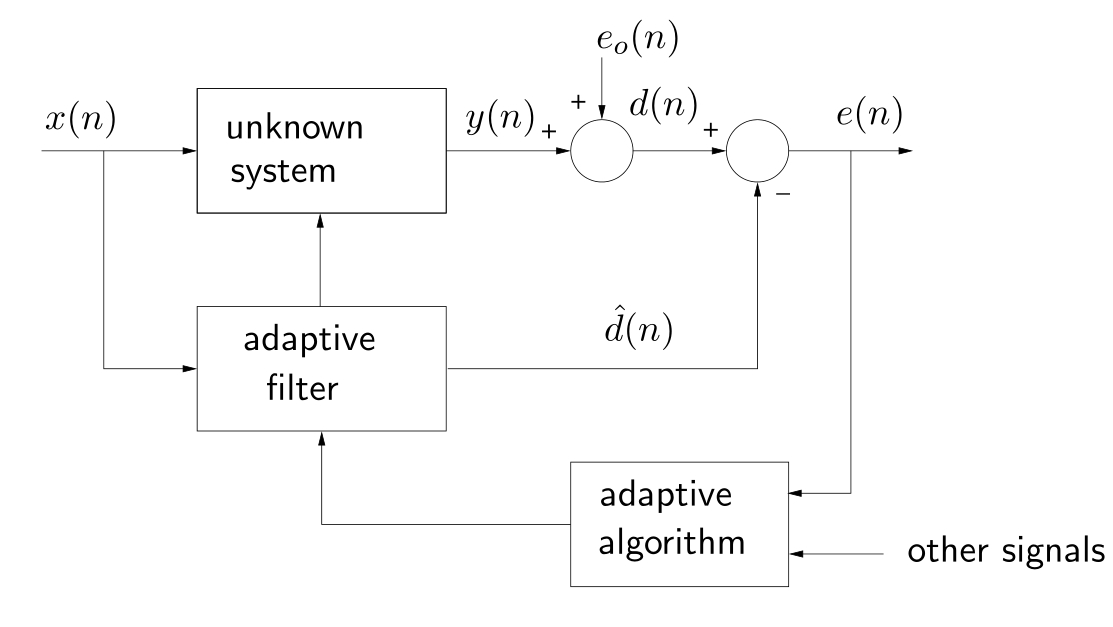
\includegraphics[scale=0.3]{SystemIdentification.jpg}
\end{center}
\end{frame}

\begin{frame}
\frametitle{Applications - System Identification}
\textcolor{red}{Channel Estimation}
\begin{itemize}
  \item Communication systems
  \item Objective: model the channel to design distortion compensation
  \item $x(n):$ training sequences
\end{itemize}
\textcolor{red}{Plant Identification}
\begin{itemize}
  \item Control systems
  \item Objective: model the plant to design a compensator
  \item $x(n):$ training sequence
\end{itemize}
\end{frame}

\section{Result}
\subsection{MATLAB Codes}

\begin{frame}[fragile,containsverbatim]
\frametitle{AffineProjection.m}
\begin{block}{API}
\begin{verbatim}
function    [outputVector,...
             errorVector,...
             coefficientVector] =
             AffineProjection(desired,input,S)
\end{verbatim}
\end{block}
\end{frame}

\begin{frame}[fragile,containsverbatim,shrink]
\begin{block}{Body}
\begin{verbatim}
for it = 1:nIterations,

    regressor(:,2:S.memoryLength+1) =
    regressor(:,1:S.memoryLength);
    regressor(:,1)                  =
    prefixedInput(it+(nCoefficients-1):-1:it);
    outputVectorApConj(:,it)        =
    (regressor')*coefficientVector(:,it);
    errorVectorApConj(:,it)         =
    conj(prefixedDesired(it+(S.memoryLength):-1:it))...
    -outputVectorApConj(:,it);
    coefficientVector(:,it+1)       =
    coefficientVector(:,it)+(S.step*regressor*...
    inv(regressor'*regressor+S.gamma*...
    eye(S.memoryLength+1))*errorVectorApConj(:,it));
end
\end{verbatim}
\end{block}
\end{frame}

\subsection{Simulation Results}
\begin{frame}
\frametitle{Learning Curve}
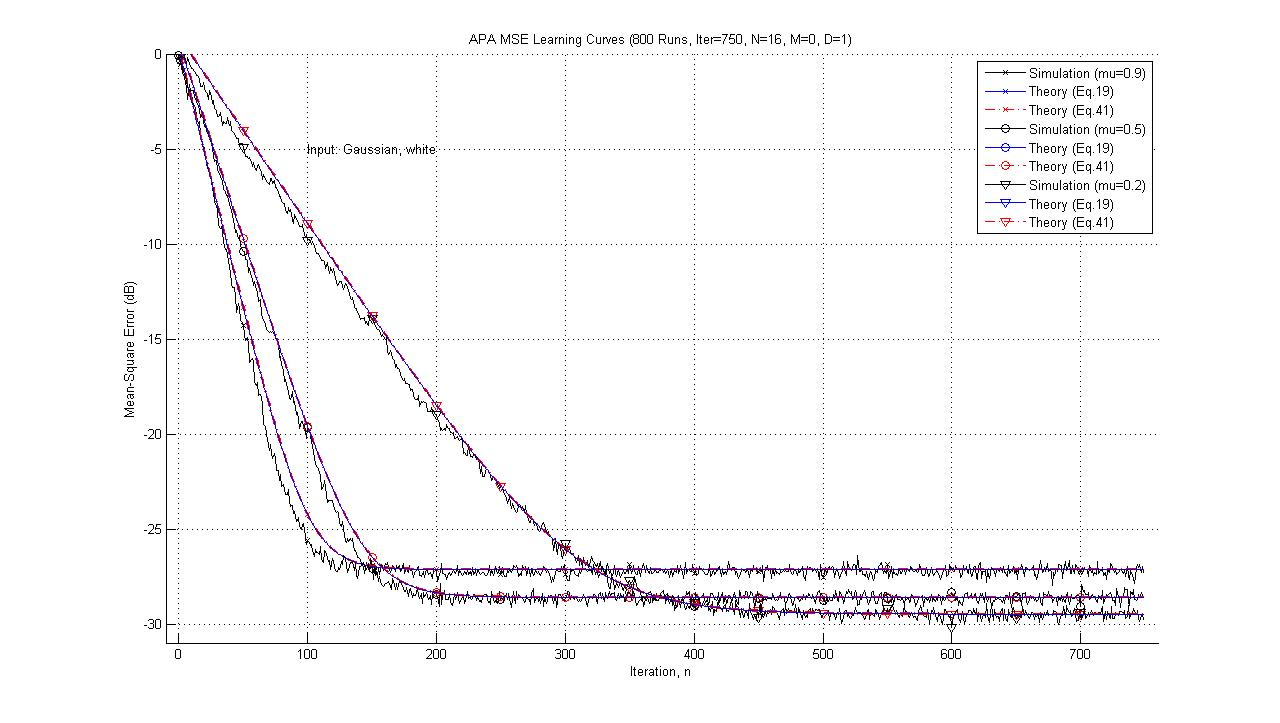
\includegraphics[scale=0.26]{Result001.jpg}
\end{frame}

\begin{frame}
\frametitle{Steady State}
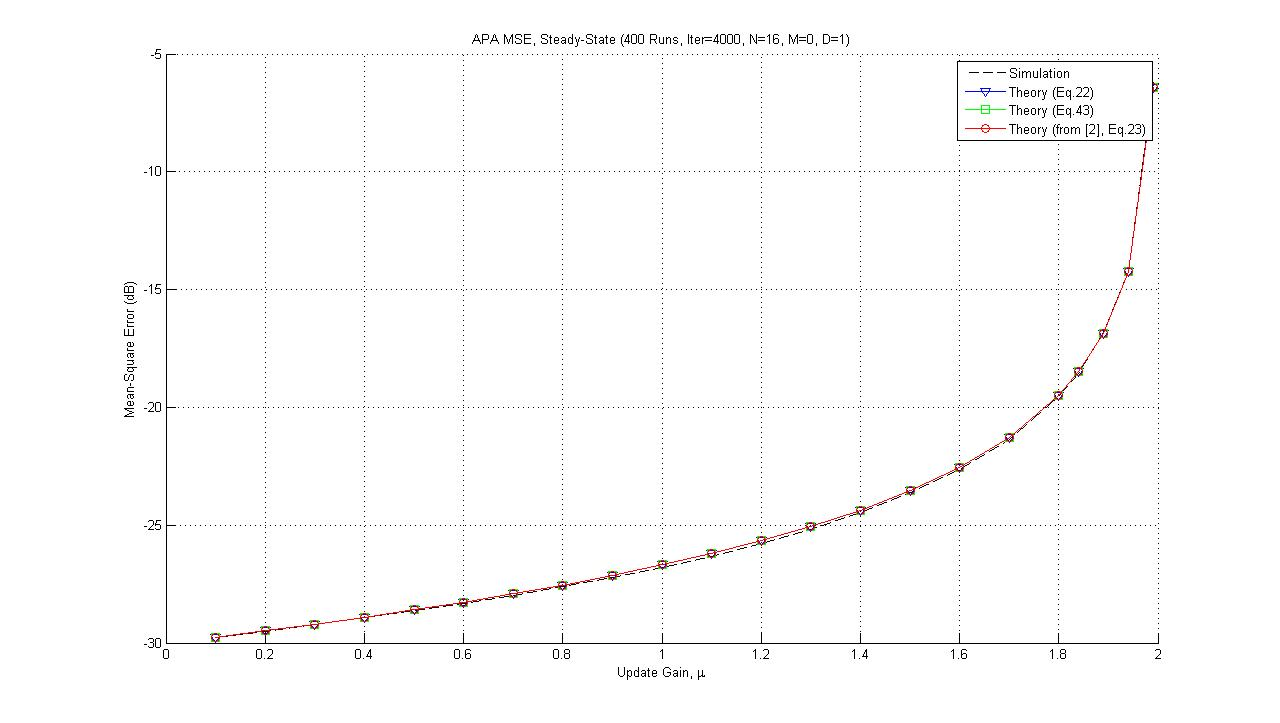
\includegraphics[scale=0.26]{Result005.jpg}
\end{frame}

\section{Further Work}
\subsection{Weight Error Update Equations}
\begin{frame}
\frametitle{Weight Error Update Equations}
% \begin{table}
% \begin{tabular}{cc}
% Algorithm & Update Equations\\
% Steepest Descent &  $\mathbf{w}(n+1)=\mathbf{w}(n)+\mu[\mathbf{p}-\mathbf{R}_{xx}\mathbf{w}(n)]$\\
%
% \end{tabular}
% \end{table}
Steepest Descent Algorithm - Stationary SOE
\begin{equation}\label{equ:SteepestDA}
  \mathbf{w}(n+1)=\mathbf{w}(n)+\mu[\mathbf{p}-\mathbf{R}_{xx}\mathbf{w}(n)]
\end{equation}
Newton Algorithm
\begin{equation}\label{equ:NetwonA}
  \mathbf{w}(n+1)=\mathbf{w}(n)-\mu\mathbf{R}^{-1}_{xx}[-\mathbf{p}+\mathbf{R}_{xx}\mathbf{w}(n)]
\end{equation}
Least Mean Squares (LMS) Algorithm
\begin{equation}\label{euq:LeastMeanSquare}
  \mathbf{w}(n+1)=\mathbf{w}(n)+\mu e(n)\mathbf{x}(n)
\end{equation}
\end{frame}

\begin{frame}
\frametitle{Weight Error Update Equations - continued}
Normalized Least Mean Square (NLMS) Algorithm
\begin{equation}\label{equ:NormalizedLeastMeanSquare}
  \mathbf{w}(n+1)=\mathbf{w}(n)+\mu\frac{e(n)\mathbf{x}(n)}
  {\mathbf{x}^{T}(n)\mathbf{x}(n)}
\end{equation}
Affine Projection (AP) Algorithm
\begin{equation}\label{equ:AffineProjectionAlgorithm}
  \mathbf{w}(n+1)=\mathbf{w}(n)+\mu\mathbf{X}(n)[\mathbf{X}^{T}(n)\mathbf{X}(n)]^{-1}\mathbf{e}(n)
\end{equation}
Recursive Least Square (RLS) Algorithm
\begin{equation}\label{equ:RecursiveLeastSquare}
  \mathbf{w}(n+1)=\mathbf{w}(n)+\mathbf{k}(n)\mathbf{e}(n)
\end{equation}
\end{frame}

\begin{frame}[fragile,shrink]
\frametitle{Weight Error Update Equations - continued}
For RLS algorithm,
\begin{equation}% \label{equ:}
  \mathbf{k}(n)=\mathbf{P}(n)\mathbf{x}(n)
\end{equation}
\begin{equation}\label{equ:RecursiveWeightUpdate}
  \mathbf{P}(n)=\lambda^{-1}\mathbf{P}(n-1)-\lambda^{-1}\mathbf{k}(n)\mathbf{x}^{T}(n)\mathbf{P}(n-1)
\end{equation}
\end{frame}

\begin{frame}[fragile]
\frametitle{Computational Complexity}
\begin{itemize}
  \item Adaptive filter with $N$ real coefficients and real signals
  \item For the AP algorithm, $K~=~P+1$
\end{itemize}
\begin{tabular}{|c|c|c|c|}

  \hline
  % after \\: \hline or \cline{col1-col2} \cline{col3-col4} ...
  Algorithm & $\times$ & $+$ & $/$ \\
  LMS & $2N+1$ & $2N$ &  \\
  NLMS & $3N+1$ & $3N$ & $1$ \\
  AP & $(K^{2}+2K)N+K^{3}+K$ & $(K^{2}+2K)N+K^{3}+K$ &  \\
  RLS & $N^{2}+5N+1$ & $N^{2}+3N$ & $1$ \\
  \hline
\end{tabular}
For $N~=~100,P~=~2$
\begin{tabular}{|c|c|c|c|c|}
  \hline
  % after \\: \hline or \cline{col1-col2} \cline{col3-col4} ...
  Algorithm & $\times$ & $+$ & $/$ & $\simeq$factor \\
  LMS & 201 & 200 &  & 1 \\
  NLMS & 301 & 300 & 1 & 1.5 \\
  AP & 1,530 & 1,536 &  & 7.5 \\
  RLS & 10,501 & 10,300 & 1 & 52.5 \\
  \hline
\end{tabular}
\end{frame}

\begin{frame}
\frametitle{Computational Complexity - continued}
Typical values for acoustic echo cancellation ($N=1024, P=2$)
\begin{center}
\begin{tabular}{|c|c|c|c|c|}
  \hline
  % after \\: \hline or \cline{col1-col2} \cline{col3-col4} ...
  Algorithm & $\times$ & $+$ & $/$ & $\simeq$factor \\
  LMS & 2,049 & 2,048 &  & 1 \\
  NLMS & 3,073 & 3,072 & 1 & 1.5 \\
  AP & 15,390 & 15,396 &  & 7.5 \\
  RLS & 1,053,697 & 1,051,648 & 1 & 514 \\
  \hline
\end{tabular}
\end{center}
\end{frame}

\subsection{Deal with Computational Complexity}
\begin{frame}
\frametitle{How to Deal with Computational Complexity?}
\begin{itemize}
  \item[$\bigstar$] Not an easy task!!!
  \item[$\bigstar$] There are "fast" versions for some algorithms (especially RLS)
  \item[$\bigstar$] What is usually not said is that...speed can bring
  \item \textcolor{red}{Instability}
  \item Increased need for \textcolor{red}{memory}
\end{itemize}
\emph{\textcolor{blue}{Most applications rely on simple solutions.}}\\
\end{frame}

\subsection{Instability \& Memory}
\begin{frame}
\frametitle{Instability}
\begin{center}
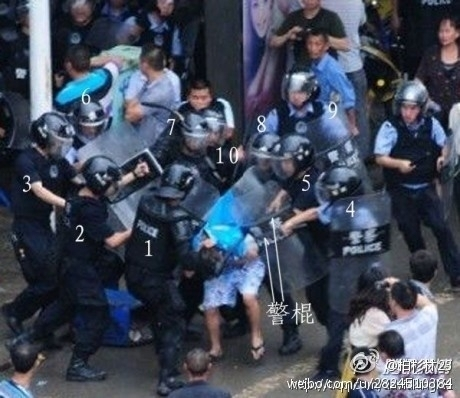
\includegraphics[scale=0.45]{Instability.jpg}
\end{center}
\end{frame}

\begin{frame}
\frametitle{Memory}
\begin{center}
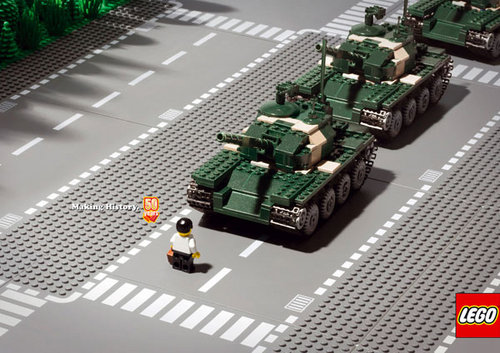
\includegraphics[scale=0.75]{Memory.jpeg}
\end{center}
\end{frame}

\subsection{Workload}
\begin{frame}
\frametitle{Workload}
\begin{center}
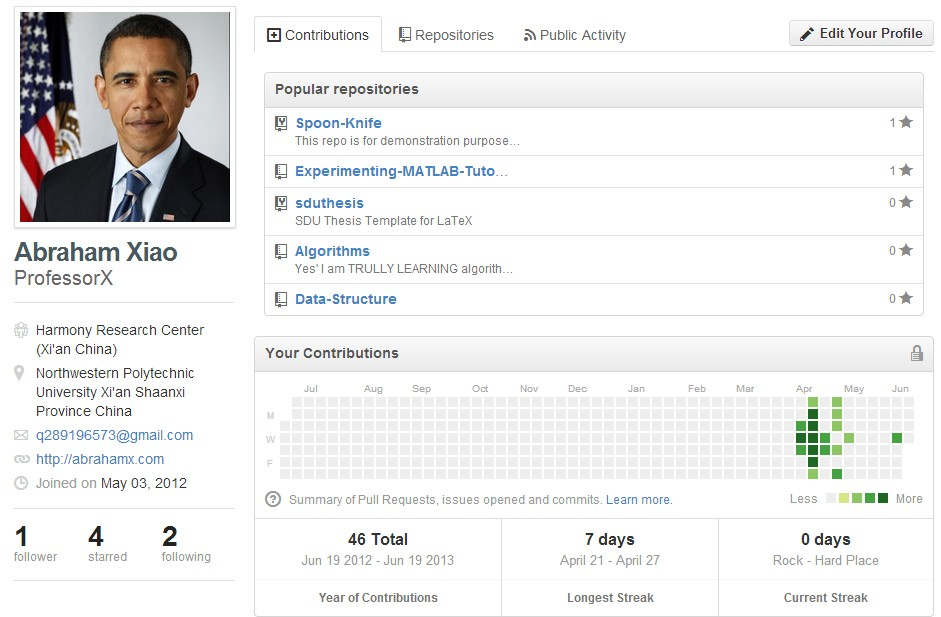
\includegraphics[scale=0.3]{Workload.jpg}
\end{center}
\end{frame}






\section{Question \& Answer}
\subsection{Open for Any Questions}
\begin{frame}
\begin{center}

\includegraphics[scale=0.45]{Question.jpg}
\end{center}
\end{frame}










\end{document} 